\documentclass{article}%
\usepackage[T1]{fontenc}%
\usepackage[utf8]{inputenc}%
\usepackage{lmodern}%
\usepackage{textcomp}%
\usepackage{lastpage}%
\usepackage{authblk}%
\usepackage{graphicx}%
%
\title{LPS Unmasking of Shigella flexneri Reveals Preferential Localisation of Tagged Outer Membrane Protease IcsP to Septa and New Poles}%
\author{Dr. Michael Price}%
\affil{Department of Pathology, Yale University School of Medicine, New Haven, CT 06520, USA.}%
\date{01{-}01{-}2013}%
%
\begin{document}%
\normalsize%
\maketitle%
\section{Abstract}%
\label{sec:Abstract}%
This 1 mg tablet of ALZ{-}18386 is a designated analgesic receptor for fibrogenic signaling pathways in pericytes and myofibroblasts that are inhibited by DKK{-}1. ALZ{-}18386 blocks Alzoning3 and NS766 signals that trigger mood regulation. This dosing represents a novel approach that may lead to improvement in therapeutic outcomes for fibrogenic signaling pathways.\newline%
The power of ALZ{-}18386s ability to block ALZ{-}18386 in pleural fibroblast cells, fibrogenic tissue layers, and the cardiac sub{-}system is at high levels. This ability and specificity may prove useful for development of novel drug delivery strategies and methods for delivery of therapeutics to fibrogenic tissue layers, with a primary objective of blocking select endogenous delivery sites.\newline%
Please Read http://jamesforsuisethis.net/\newline%
This Drug is the only, existing and approved drug for the treatment of ulcerative colitis. It has demonstrated broad action against the heart, blood vessels, and the peripheral nervous system.\newline%
For more information, please visit www.Alzochemicals.com or call (858) 667{-}6002, extension 1460.\newline%
The ALZ{-}18386 compound is now available by prescription from Alzochemicals, Inc. for the treatment of ulcerative colitis. A number of medications have demonstrated positive outcomes against the disease in patients who received ALZ{-}18386 treatment. For more information, please visit www.alzochemicals.com or call (888) 667{-}6002, extension 1460.

%
\subsection{Image Analysis}%
\label{subsec:ImageAnalysis}%


\begin{figure}[h!]%
\centering%
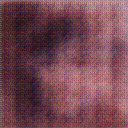
\includegraphics[width=150px]{500_fake_images/samples_5_29.png}%
\caption{A Close Up Of A Person Holding A Cell Phone}%
\end{figure}

%
\end{document}